\chapter{Cross-loop Optimization of Arithmetic Intensity for Finite Element Local Assembly}
\label{ch:coffee}

\section{Introduction and Motivations}
In many fields such as computational fluid dynamics, computational electromagnetics and structural mechanics, phenomena are modelled by partial differential equations (PDEs). Numerical techniques, like the finite volume method and the finite element method, are widely employed to approximate solutions of these PDEs. Unstructured meshes are often used to discretize the computational domain, since they allow an accurate representation of complex geometries. The solution is sought by applying suitable numerical operations, or
kernels, to the entities of a mesh, such as edges, vertices, or cells. On standard clusters of multicores, typically, a kernel is executed sequentially by a thread, while parallelism is achieved by partitioning the mesh and assigning each partition to a different node or thread. Such an execution model, with minor variations, is adopted, for example, in \cite{pyop2isc}, \cite{Fenics}, \cite{fluidity_manual_v4}, \cite{lizst}.

The time required to apply the numerical kernels is a major issue, since the equation domain needs to be discretized into an extremely large number of cells to obtain a satisfactory approximation of the PDE, possibly of the order of trillions, as in \cite{Rossinelli2013}. For example, it has been well established that mesh resolution is critical in the accuracy of numerical weather forecasts. However, operational forecast centers have a strict time limit in which to produce a forecast - 60 minutes in the case of the UK Met Office. Producing efficient kernels has a direct scientific payoff in higher resolution, and therefore more accurate, forecasts. Computational cost is a dominant problem in computational science simulations, especially for those based on finite elements, which are the subject of this work. In this chapter, we address, in particular, the well-known problem of optimizing the local assembly phase of the finite element method, which can be responsible for a significant fraction of the overall computation run-time, often in the range 30-60$\%$ \citep{francis}, \citep{quadrature-olegaard}, \citep{petsc-integration-gpu}, \citep{tensor-kirby}. 

During the assembly phase, the solution of the PDE is approximated by executing a problem-specific kernel over all cells, or elements, in the discretized domain. We restrict our focus to relatively low order finite element methods, in which an assembly kernel's working set is usually small enough to fit the L1 cache. Low order methods are by no means exotic: they are employed in a wide variety of fields, including climate and ocean modeling, computational fluid dynamics, and structural mechanics. The efficient assembly of high order methods such as the spectral element method \citep{spencer} requires a significantly different loop nest structure. High order methods are therefore excluded from our study.

An assembly kernel is characterized by the presence of an affine, often non-perfect loop nest, in which individual loops are rather small: their trip count rarely exceeds 30, and may be as low as 3 for low order methods. In the innermost loop, a problem-specific, compute intensive expression evaluates a two dimensional array, representing the result of local assembly in an element of the discretized domain. With such a kernel structure, we focus on aspects like the minimization of floating-point operations, register allocation and instruction-level parallelism, especially in the form of SIMD vectorization.

We aim to maximize our impact on the platforms that are realistically used for finite element applications, so we target conventional CPU architectures rather than GPUs. 
The key limiting factor to the execution on GPUs is the stringent memory requirements. Only relatively small problems fit in a GPU memory, and support for distributed GPU execution in general purpose finite element frameworks is minimal. There has been some research on adapting local assembly to GPUs (mentioned later), although it differs from ours in several ways, including: (i) not relying on automated code generation from a domain-specific language (explained next), (ii) testing only very low order methods, (iii) not optimizing for cross-loop arithmetic intensity (the goal is rather effective multi-thread parallelization). In addition, our code transformations would drastically impact the GPU parallelization strategy, for example by increasing a thread's working set. For all these reasons, a study on extending the research to GPU architectures is beyond the scope of this work. In Section~\ref{sec:generality}, however, we provide some intuitions about this research direction.

Achieving high-performance on CPUs is non-trivial. The complexity of the mathematical expressions, often characterized by a large number of operations on constants and small matrices, makes it hard to determine a single or specific sequence of transformations that is successfully applicable to all problems. Loop trip counts are typically small and can vary significantly, which further exacerbates the issue. We will show that traditional vendor compilers, such as \emph{GNU's} and \emph{Intel's}, fail at exploiting the structure inherent such assembly expressions. Polyhedral-model-based source-to-source compilers, for instance~\cite{pluto}, can apply aggressive loop optimizations, such as tiling, but these are not particularly helpful in our context, as explained next. 

We focus on optimizing the performance of local assembly operations produced by automated code generation. This technique has been proved successful in the context of the FEniCS~\citep{Fenics} and Firedrake~\citep{firedrake-code} projects, become incredibly popular over the last years. In these frameworks, a mathematical model is expressed at high-level by means of a domain-specific language and a domain-specific compiler is used to produce a representation of local assembly operations (e.g. C code). \textit{Our aim is to obtain close-to-peak performance in all of the local assembly operations that such frameworks can produce}. Since the domain-specific language exposed to the users provide as constructs generic differential operators, an incredibly vast set of PDEs, possibly arising in completely different domains, can be expressed and solved. A compiler-based approach is, therefore, the only reasonable option to the problem of optimizing local assembly operations. 

Several studies have already tackled local assembly optimization in the context of automated code generation. In~\cite{quadrature-olegaard}, it is shown how this technique can be leveraged to introduce domain-specific optimizations, which a user cannot be expected to write ``by hand''. \cite{tensor-kirby} and~\cite{francis} have studied, instead, different optimization techniques based on a mathematical reformulation of the local assembly operations. The same problem has been addressed recently also for GPU architectures, for instance in~\cite{petsc-integration-gpu},~\cite{klockner-dg}, and~\cite{bana-ho-fem}. With our study, we make clear step forward by showing that different PDEs, on different platforms, require distinct sets of transformations if close-to-peak performance must be reached, and that low-level, domain-aware code transformations are essential to maximize instruction-level parallelism and register locality. As discussed in the following sections, our optimization strategy is quite different from those in previous work, although we reuse and leverage some of the ideas formulated in the available literature. 

We present a novel structured approach to the optimization of automatically-generated local assembly kernels. We argue that for complex, realistic PDEs, peak performance can be achieved only by passing through a two-step optimization procedure: 1) expression rewriting, to minimize floating point operations, 2) and code specialization, to ensure effective register utilization and instruction-level parallelism, especially SIMD vectorization. 

Expression rewriting consists of a framework capable of minimizing arithmetic intensity and optimize for register pressure. Our contribution is twofold:
\begin{itemize}
\item \emph{Rewrite rules for assembly expressions}. The goal is to the reduce the computational intensity of local assembly kernels by rescheduling arithmetic operations based on a set of rewrite rules. These aggressively exploit associativity, distributivity, and commutativity of operators to expose loop-invariant sub-expressions and SIMD vectorization opportunities to the code specialization stage. While rewriting an assembly expression, domain knowledge is used in several ways, for example to avoid redundant computation.
\item \emph{An algorithm to deschedule useless operations}. Relying on symbolic execution, this algorithm restructures the code so as to skip useless arithmetic operations, for example multiplication by scalar quantities which are statically known to be zero. One problem is to transform the code while preserving code vectorizability, which is solved by resorting to domain-knowledge. 
\end{itemize}

Code specialization's goal is to apply transformations to maximize the exploitation of the underlying platform's resources, e.g. SIMD lanes. We provide a number of contributions:
\begin{itemize}
\item \emph{Padding and data alignment}. The small size of the loop nest (integration, test, and trial functions loops) require all of the involved arrays to be padded to a multiple of the vector register length so as to maximize the effectiveness of SIMD code. Data alignment can be enforced as a consequence of padding. 
\item \emph{Vector-register Tiling}. Blocking at the level of vector registers, which we perform exploiting the specific memory access pattern of the assembly expressions (i.e. a domain-aware transformation), improves data locality beyond traditional unroll-and-jam optimizations. This is especially true for relatively high polynomial order (i.e. greater than 2) or when pre-multiplying functions are present.
\item \emph{Expression Splitting}. In certain assembly expressions the register pressure is significantly high: when the number of basis functions arrays (or, equivalently, temporaries introduced by loop-invariant code motion) and constants is large, spilling to L1 cache is a consequence for architectures with a relatively low number of logical registers (e.g. 16/32). We exploit sum's associativity to ``split'' the assembly expression into multiple sub-expressions, which are computed individually.
\item \emph{An algorithm to generate calls to BLAS routines}.
\item \emph{Autotuning}. We implement a model-driven, dynamic autotuner that transparently evaluates multiple sets of code transformations to determine the best optimization strategy for a given PDE. The main challenge here is to build, for a generic problem, a reasonably small search space that comprises most of the effective code variants.
\end{itemize} 

Expression rewriting and code specialization have been implemented in a compiler, COFFEE\footnote{COFFEE stands for COmpiler For Finit Element local assEmbly.}, fully integrated with the Firedrake framework~\cite{Luporini}. Besides separating the mathematical domain, captured by a domain-specific compiler at an higher level of abstraction, from the optimization process, COFFEE also aims to be platform-agnostic. The code transformations occur on an intermediate representation of the assembly operation, which is ultimately translated into platform-specific code. Domain knowledge is exploited in two ways: for simplifying the implementation of code transformations and to make them extremely effective. Domain knowledge is conveyed to COFFEE from the higher level through suitable annotations attached to the input. For example, when the input is in the form of an abstract syntax tree produced by the higher layer, specific nodes are decorated so as to drive the optimization process. Although COFFEE has been thought of as a multi-platform optimizing compiler, our performance evaluation so far has been restricted to standard CPU platforms only. We emphasize once more, however, that all of the transformations applicable would work on generic accelerators as well.

To demonstrate the effectiveness of our approach, we provide an extensive and unprecedented performance evaluation across a number of real-world PDEs of increasing complexity, including some based on complex hyperelasticity models. We characterize our problems by varying polynomial order of the employed function spaces and number of so called pre-multiplying functions. To clearly distinguish the improvements achieved by COFFEE, we will compare, for each examined PDE, four sets of code variants: 1) unoptimized code, i.e. a local assembly routine as returned from the domain-specific compiler; 2) code optimized by FEniCS, i.e. the work in~\cite{quadrature-olegaard}; 3) code optimized by expression rewriting and code specialization as described in this paper. Notable performance improvements of 3) over 1) and 2) are reported and discussed.

\section{Preliminaries}
\label{sec:coffee-preliminaries}
In this section, the basic concepts sustaining the finite element method are summarized. The notation adopted in~\cite{quadrature-olegaard} and~\cite{francis} is followed. At the end of this section, the reader is expected to understand what local assembly represents and how an implementation can be derived starting from a mathematical specification of the finite element problem. 

\subsection{Overview of the Finite Element Method}
We consider the weak formulation of a linear variational problem
\begin{equation}
\begin{split}
Find\ u\ \in U\ such\ that \\
a(u, v) = L(v), \forall v \in V
\end{split}
\end{equation}
where $a$ and $L$ are called bilinear and linear form, respectively. The set of \textit{trial} functions $U$ and the set of \textit{test} functions $V$ are discrete function spaces. For simplicity, we assume $U = V$ and $\lbrace \phi_i \rbrace$ be the set of basis functions spanning $U$. The unknown solution $u$ can be approximated as a linear combination of the basis functions $\lbrace \phi_i \rbrace$. From the solution of the following linear system it is possible to determine a set of coefficients to express $u$
\begin{equation}
A\textbf{u} = b
\end{equation}
in which $A$ and $b$ discretize $a$ and $L$ respectively:
\begin{equation}
\centering
\begin{split}
A_{ij} = a(\phi_i(x), \phi_j(x)) \\
b_i = L(\phi_i(x))
\end{split}
\end{equation}
The matrix $A$ and the vector $b$ are computed in the so called assembly phase. Then, in a subsequent phase, the linear system is solved, usually by means of an iterative method, and $\textbf{u}$ is eventually evaluated. 

We focus on the assembly phase, which is often characterized as a two-step procedure: \textit{local} and \textit{global} assembly. Optimizing the performance of local assembly is the subject of the research. Local assembly consists of computing the contributions that an element in the discretized domain provide to the approximated solution of the equation. Global assembly, on the other hand, is the process of suitably ``inserting'' such contributions in $A$ and $b$. 

\subsection{Quadrature Representation for Finite Element Local Assembly}
\label{sec:quadrature-rep}
Without loss of generality, we illustrate local assembly in a concrete example, the evaluation of the local element matrix for a Laplacian operator. Consider the weighted Laplace equation
\begin{equation}
- \nabla \cdot (w \nabla u) = 0
\end{equation}
in which $u$ is unknown, while $w$ is prescribed. The bilinear form associated with the weak variational form of the equation is:
\begin{equation}
a(v, u) = \int_\Omega w \nabla v \cdot \nabla u\ \mathrm{d}x
\end{equation}
The domain $\Omega$ of the equation is partitioned into a set of cells (elements) $T$ such that $\bigcup T = \Omega$ and $\bigcap T = \emptyset$. By defining $\lbrace \phi_i^K \rbrace$ as the set of local basis functions spanning $U$ on the element $K$, we can express the local element matrix as
\begin{equation}
\label{eq:stiffness}
A_{ij}^K = \int_K w \nabla \phi_i^K \cdot \nabla \phi_j^K\ \mathrm{d}x
\end{equation}
The local element vector $L$ can be determined in an analogous way starting from the linear form associated with the weak variational form of the equation. 

Quadrature schemes are conveniently used to numerically evaluate $A_{ij}^K$. For convenience, a reference element $K_0$ and an affine mapping $F_K : K_0 \rightarrow K$ to any element $K \in T$ are introduced. This implies a change of variables from reference coordinates $X_0$ to real coordinates $x = F_K (X_0)$ is necessary any time a new element is evaluated. The numerical integration routine based on quadrature representation over an element $K$ can be expressed as follows
\begin{equation}
\label{eq:quadrature}
\scriptsize
A_{ij}^K = \sum_{q=1}^N \sum_{\alpha_3=1}^n \phi_{\alpha_3}(X^q)w_{\alpha_3} \sum_{\alpha_1=1}^d \sum_{\alpha_2=1}^d \sum_{\beta=1}^d \frac{\partial X_{\alpha_1}}{\partial x_{\beta}} \frac{\partial \phi_i^K(X^q)}{\partial X_{\alpha_1}} \frac{\partial X_{\alpha_2}}{\partial x_{\beta}} \frac{\partial \phi_j^K(X^q)}{\partial X_{\alpha_2}} det F_K' W^q
\end{equation}
where $N$ is the number of integration points, $W^q$ the quadrature weight at the integration point $X^q$, $d$ is the dimension of $\Omega$, $n$ the number of degrees of freedom associated to the local basis functions, and $det$ the determinant of the Jacobian matrix used for the aforementioned change of coordinates.  

In the next sections, we will often refer to the local element matrix evaluation, such as Equation~\ref{eq:quadrature} for the weighted Lapalce operator, as the \textit{assembly expression} deriving from the weak variational problem.

\subsection{Implementation of Quadrature-based Local Assembly}
\subsubsection{From Math to Code}
We have explained that local assembly is the computation of contributions of a specific cell in the discretized domain to the linear system which yields the PDE solution. The process consists of numerically evaluating problem-specific integrals to produce a matrix and a vector (only the derivation of the matrix was shown in Section~\ref{sec:quadrature-rep}), whose sizes depend on the order of the method. This operation is applied to all cells in the discretized domain (mesh).

We consider again the weighted Laplace example of the previous section. A C-code implementation of Equation~\ref{eq:quadrature} is illustrated in Listing~\ref{code:weighted-laplace}. The values at the various quadrature points of basis functions ($\phi$) derivatives are tabulated in the FE0$\_$D10 and FE0$\_$D01 arrays. The summation along quadrature points $q$ is implemented by the \emph{i} loop, whereas the one along $\alpha_3$ is represented by the \emph{r} loop. In this example, we assume $d=2$ (2D mesh), so the summations along $\alpha_1$, $\alpha_2$ and $\beta$ have been straightforwardly expanded in the expression that evaluates the local element matrix $A$. 

\begin{algorithm}
\scriptsize
\SetAlgorithmName{LISTING}{}

\KwSty{void} weighted$\_$laplace(\KwSty{double} A[3][3], \KwSty{double} **coordinates, \KwSty{double} **w) \\
$\lbrace$ \\
~~  // Compute Jacobian \\
~~  \KwSty{double} J[4]; \\
~~  compute$\_$jacobian$\_$triangle$\_$2d(J, coordinates); \\
~~\\
~~  // Compute Jacobian inverse and determinant \\
~~  \KwSty{double} K[4]; \\
~~  \KwSty{double} detJ; \\
~~  compute$\_$jacobian$\_$inverse$\_$triangle$\_$2d(K, detJ, J); \\
~~  \KwSty{const double} det = fabs(detJ); \\
~~\\
~~  // Quadrature weights \\
~~  \KwSty{static const double} W1[1] = {0.5}; \\
~~\\
~~  // Basis functions \\
~~  \KwSty{static const double} FE0$\_$D10[1][3] = $\lbrace\lbrace$ -0.999999999999999, ...$\rbrace\rbrace$ ;\\
~~  \KwSty{static const double} FE0$\_$D01[1][3] = $\lbrace\lbrace$ -1.0, ...$\rbrace\rbrace$ ;\\
~~  \KwSty{static const double} FE0[1][3] = $\lbrace\lbrace$ 0.333333333333333, ...$\rbrace\rbrace$ ;\\
~~\\
~~  \KwSty{for} (\KwSty{int} i = 0; i < 6; ++i)\\
~~  $\lbrace$\\
~~~~  \KwSty{double} F0  = 0.0;\\
~~~~  \KwSty{for} (\KwSty{int} r  = 0; r < 3; ++r)\\
~~~~~~  F0 += (w[r][0] * FE0[i][r]);\\
~~\\
~~~~  \KwSty{for} (\KwSty{int} j = 0; j < 3; ++j)\\
~~~~~~    \KwSty{for} (\KwSty{int} k = 0; k < 3; ++k)\\
~~~~~~~~      A[j][k] += (\underline{(}\textbf{(}((K[1]*FE0$\_$D10[i][k])+(K[3]*FE0$\_$D01[i][k])) * \\
~~~~~~~~~~~~~~~~~~~~~~~~~~~~((K[1]*FE0$\_$D10[i][j])+(K[3]*FE0$\_$D01[i][j]))\textbf{)} + \\
~~~~~~~~~~~~~~~~~~~~~~~~~~~~\textbf{(}((K[0]*FE0$\_$D10[i][k])+(K[2]*FE0$\_$D01[i][k])) * \\
~~~~~~~~~~~~~~~~~~~~~~~~~~~~((K[0]*FE0$\_$D10[i][j])+(K[2]*FE0$\_$D01[i][j]))\textbf{)}\underline{)}*det*W1[i]*F0);\\
~~  $\rbrace$\\
$\rbrace$
\caption{A possible implementation of Equation~\ref{eq:quadrature} assuming a 2D triangular mesh and polynomial order $p=2$ Lagrange basis functions.}
\label{code:weighted-laplace}
\end{algorithm}

More complex assembly expressions, due to the employment of particular differential operators in the original PDE, are obviously possible. Intuitively, as the complexity of the PDE grows, the implementation of local assembly becomes increasingly more complicated. This fact is actually the real motivation behind reasearch in automated code generation techniques, such as those used by state-of-the-art frameworks like FEniCS and Firedrake. Automated code generation allows scientists to express the finite element specfication using a domain-specific language resembling mathematical notation, and obtain with no effort a semantically correct implementation of local assembly. The research in the present work is about making such an implementation also extremely effective, in terms of run-time performance, on standard CPU architectures. 

\begin{algorithm}
\scriptsize
\SetAlgorithmName{LISTING}{}

// This is a Firedrake construct (\textbf{not} an UFL's) to instantiate a 2D mesh.\\
mesh = UnitSquareMesh(size, size)\\
// FunctionSpace also belongs to the Firedrake language \\
V = FunctionSpace(mesh, "Lagrange", 2)\\
u = \KwSty{TrialFunction}(V)\\
v = \KwSty{TestFunction}(V)\\
weight = \KwSty{Function(V)}.\KwSty{assign}(value)\\
a = weight\KwSty{*}\KwSty{dot}(\KwSty{grad}(v), \KwSty{grad}(u))\KwSty{*dx}
\caption{UFL specification of the weighted Laplace equation for polynomial order $p=2$ Lagrange basis functions.}
\label{code:weighted-laplace-ufl}
\end{algorithm}

The domain-specific language used by Firedrake and FEniCS to express finite element problems is the Unified Form Language (UFL) \citep{ufl}. Listing~\ref{code:weighted-laplace-ufl} shows a possible UFL implementation for the weighted Laplace form. Note the resemblance of \emph{a = weight*...} with Equation~\ref{eq:stiffness}. A form compiler translates UFL code into the C code shown in Listing~\ref{code:weighted-laplace}. We will describe these aspects carefully in Section~\ref{sec:coffee-implementation}; for the moment, this level of detail sufficies to open a discussion on how to optimize local assembly kernels arising from generic partial differential equations.

\subsubsection{Other Examples and Motivations for Optimizations}

\begin{figure}
\begin{alltt}
\scriptsize
\textbf{Input:} element matrix (2D array, initialized to 0), coordinates (array), 
       coefficients (array, e.g. velocity)
\textbf{Output:} element matrix (2D array)
- Compute Jacobian from coordinates
- Define basis functions
- Compute element matrix in an affine loop nest
\end{alltt}
\caption{Structure of a local assembly kernel}
\label{code:general-structure}
\end{figure}

%The code transformations described in this work are also
%generalizable to non-Firedrake assembly kernels, provided that the
%same numerical integration algorithm is employed.

The structure of a local assembly kernel can be generalized as in Figure~\ref{code:general-structure}. The inputs are a zero-initialized two dimensional array used to store the element matrix, the element's coordinates in the discretized domain, and coefficient fields, for instance indicating the values of velocity or pressure in the element. The output is the evaluated element matrix. The kernel body can be logically split into three parts:
\begin{enumerate}
  \item Calculation of the Jacobian matrix, its determinant and its
    inverse required for the aforementioned change of coordinates from
    the reference element to the one being computed.
  % FIXME: this rather hand-wavy and not technically correct
  \item Definition of basis functions used to interpolate fields at the
    quadrature points in the element. The choice of basis functions is
    expressed in UFL directly by users. In the generated code, they are
    represented as global read-only two dimensional arrays (i.e., using
    \texttt{static const} in C) of double precision floats.
  \item Evaluation of the element matrix in an affine loop nest, in which
    the integration is performed.
\end{enumerate}
Table~\ref{table:map-name-letters} shows the variable names we will use in the upcoming code snippets to refer to the various kernel objects.

\begin{table}
\scriptsize
\begin{center}
\begin{tabulary}{1.0\columnwidth}{C|C|C}
\hline
Object name & Type & Variable name(s) \\\hline
Determinant of the Jacobian matrix & double & det  \\
Inverse of the Jacobian matrix & double & K1, K2, ... \\
Coordinates & double** & coords\\
Fields (coefficients) & double** & w \\
Numerical integration weights & double[] & W \\
Basis functions (and derivatives) & double[][] & X, Y, X1, ... \\
Element matrix & double[][] & A\\ \hline
\end{tabulary}
\end{center}
\caption{Type and variable names used in the various listings to identify local assembly objects.}
\label{table:map-name-letters}
\end{table}

%JUNK SENTENCES: Since only the values assumed at the integration
%points are needed to compute the element matrix, a basis function is
%implemented as a two dimensional array of double precision
%floats. The same basis functions can be used to evaluate all element
%matrices, provided that a suitable change of coordinates from a
%``reference'' element to a real one is performed. Therefore, basis
%functions are declared in the kernel body as global read-only arrays
%(i.e., using \texttt{static const} in C), rather than passed as
%function parameters. Basis functions are chosen at the UFL layer
%based on the problem being solved, so they are actually an input to
%the code generator.

\begin{algorithm}[t]
\scriptsize
\SetAlgorithmName{LISTING}{}

\KwSty{void} helmholtz(\KwSty{double} A[3][3], \KwSty{double} **coords) $\lbrace$\\
~~// K, det = Compute Jacobian (coords) \\
~~\\
~~\KwSty{static const double} W[3] = $\lbrace$...$\rbrace$\\
~~\KwSty{static const double} X$\_$D10[3][3] = $\lbrace\lbrace$...$\rbrace\rbrace$\\
~~\KwSty{static const double} X$\_$D01[3][3] = $\lbrace\lbrace$...$\rbrace\rbrace$\\
~~\\
~~\KwSty{for} (\KwSty{int} i = 0; i$<$3; i++) \\
~~~~\KwSty{for} (\KwSty{int} j = 0; j$<$3; j++) \\
~~~~~~\KwSty{for} (\KwSty{int} k = 0; k$<$3; k++) \\
~~~~~~~~A[j][k] += ((Y[i][k]*Y[i][j]+\\
~~~~~~~~~~~+((K1*X$\_$D10[i][k]+K3*X$\_$D01[i][k])*(K1*X$\_$D10[i][j]+K3*X$\_$D01[i][j]))+\\
~~~~~~~~~~~+((K0*X$\_$D10[i][k]+K2*X$\_$D01[i][k])*(K0*X$\_$D10[i][j]+K2*X$\_$D01[i][j])))*\\
~~~~~~~~~~~*det*W[i]);\\
$\rbrace$
\caption{Local assembly implementation for a Helmholtz problem on a 2D mesh using polynomial order $p=1$ Lagrange basis functions.}
\label{code:helmholtz}
\end{algorithm}

\begin{algorithm}[t]
\scriptsize
\SetAlgorithmName{LISTING}{}

\KwSty{void} burgers(\KwSty{double} A[12][12], \KwSty{double} **coords, \KwSty{double} **w) $\lbrace$\\
~~// K, det = Compute Jacobian (coords) \\
~~\\
~~\KwSty{static const double} W[5] = $\lbrace$...$\rbrace$\\
~~\KwSty{static const double} X1$\_$D001[5][12] = $\lbrace\lbrace$...$\rbrace\rbrace$\\
~~\KwSty{static const double} X2$\_$D001[5][12] = $\lbrace\lbrace$...$\rbrace\rbrace$\\
~~//11 other basis functions definitions.\\
~~...\\
~~\KwSty{for} (\KwSty{int} i = 0; i$<$5; i++) $\lbrace$\\
~~~~\KwSty{double} F0 = 0.0;\\
~~~~//10 other declarations (F1, F2,...)\\
~~~~...\\
~~~~\KwSty{for} (\KwSty{int} r = 0; r$<$12; r++) $\lbrace$\\
~~~~~~F0 += (w[r][0]*X1$\_$D100[i][r]);\\
~~~~~~//10 analogous statements (F1, F2, ...)\\
~~~~~~...\\
~~~~$\rbrace$\\
~~~~\KwSty{for} (\KwSty{int} j = 0; j$<$12; j++) \\
~~~~~~\KwSty{for} (\KwSty{int} k = 0; k$<$12; k++) \\
~~~~~~~~A[j][k] += (..(K5*F9)+(K8*F10))*Y1[i][j])+\\
~~~~~~~~~+(((K0*X1$\_$D100[i][k])+(K3*X1$\_$D010[i][k])+(K6*X1$\_$D001[i][k]))*Y2[i][j]))*F11)+\\
~~~~~~~~~+(..((K2*X2$\_$D100[i][k])+...+(K8*X2$\_$D001[i][k]))*((K2*X2$\_$D100[i][j])+...+(K8*X2$\_$D001[i][j]))..)+\\
~~~~~~~~~+ $<$roughly a hundred sum/muls go here$>$)..)*\\
~~~~~~~~~*det*W[i]);\\
~~$\rbrace$ \\
$\rbrace$
\caption{Local assembly implementation for a Burgers problem on a 3D mesh using polynomial order $p=1$ Lagrange basis functions.}
\label{code:burgers}
\end{algorithm}

The actual complexity of a local assembly kernel depends on the finite element problem being solved. In simpler cases, the loop nest is perfect, has short trip counts (in the range 3--15), and the computation reduces to a summation of a few products involving basis functions. An example is provided in Listing~\ref{code:helmholtz}, which shows the assembly kernel for a Helmholtz problem using Lagrange basis functions on 2D elements with polynomial order $p=1$. In other scenarios, for instance when solving the Burgers equation, the number of arrays involved in the computation of the element matrix can be much larger. The assembly code is given in Listing~\ref{code:burgers} and contains 14 unique arrays that are accessed, where the same array can be referenced multiple times within the same expression. This may also require the evaluation of constants in outer loops (called $F$ in the code) to act as scaling factors of arrays. Trip counts grow proportionally to the order of the method and arrays may be block-sparse.

In general, the variations in the structure of mathematical expressions and in loop trip counts (although typically limited to the order of tens of iterations) that different equations show, render the optimization process challenging, requiring distinct sets of transformations to bring performance closest to the machine peak. For example, the Burgers problem, given the large number of arrays accessed, suffers from high register pressure, whereas the Helmholtz equation does not. Moreover, arrays in Burgers are block-sparse due to the use of vector-valued basis functions (we will elaborate on this in the next sections). These few aspects (we could actually find more) already intuitively suggests that the two problems require a different treatment, based on an in-depth analysis of both data and iteration spaces. Furthermore, domain knowledge enables transformations that a general-purpose compiler could not apply, making the optimization space even larger. In this context, our goal is to understand the relationship between distinct code transformations, their impact on cross-loop arithmetic intensity, and to what extent their composability is effective in a wide class of real-world equations and architectures.

We also note that despite the infinite variety of assembly kernels that frameworks like FEniCS and Firedrake can generate, it is still possible to identify common domain-specific traits that are potentially exploitable for our optimization strategy. These include: 1) memory accesses along the three loop dimensions are always unit stride; 2) the \texttt{j} and \texttt{k} loops are interchangeable, whereas interchanges involving the $i$ loop require pre-computation of values (e.g. the $F$ values in Burgers) and introduction of temporary arrays (explained next); 3) depending on the problem being solved, the \texttt{j} and \texttt{k} loops could iterate along the same iteration space; 4) most of the sub-expressions on the right hand side of the element matrix computation depend on just two loops (either \texttt{i}-\texttt{j} or \texttt{i}-\texttt{k}). In the following sections we show how to exploit these observations to define a set of systematic, composable optimizations.

%TODO: more observations are needed here: e.g. linear algebra operations...

\section{Overview of the Optimization Strategy}

To generate high performance implementation of local assembly kernels, assembly expressions must be optimized with regards to three interrelated aspects: 
\begin{itemize}
\item arithmetic intensity
\item instruction-level parallelism
\item data locality
\end{itemize}
Three conceptually distinct kind of transformations can be individuated, which we refer to as \textit{expression rewriting}, \textit{code specialization}, and \textit{general-purpose optimizations}. Expression rewriting mainly targets arithmetic intensity by transforming the assembly expression (and its enclosing loop nest) so as to minimize the number of floating point operations required to evaluate the local element matrix. Code specialization is tailored to optimizing for instruction-level parallelism, particularly SIMD vectorization, and data (register) locality. Both classes of transformations are inspired by the inherent structure of local assembly code and make use of domain knowledge: as elaborated in the next sections, these two aspects are the core motivations for which standard general-purpose compilers fail at maximizing the performance of local assembly kernels. The third class of transformations is about general-purpose optimizations; that is, generic, well-known techniques for improving code performance, such as loop unrolling or loop interchange, that for some reasons are not applied by the compiler generating machine code, but potentially useful in certain equations.

In Sections~\ref{sec:coffee-expr-rewrite}--\ref{sec:coffee-genpurp-opts}, these classes of code transformations are presented. In Section~\ref{sec:coffee-implementation}, it is explained that their application to local assembly kernels must follow a specific order to ensure the correctness of the resulting code. Some effort was invested in ensuring that optimizations at stage $i$ (e.g. expression rewriting) would not break any further optimization opportunity at stage $i+1$ (code specialization). The theory and the implementation of a technique to select the optimal combination of transformations for a given equation are finally discussed.

% Need to mention composability here

\section{Expression Rewriting}
\label{sec:coffee-expr-rewrite}

Expression rewriting is about exploiting properties of operators such as associativity, distributivity, and commutativity, to minimize arithmetic intensity, expose code vectorization opportunities, and optimize the register pressure in the various levels of the assembly loop nest. There are many possibilities of rewriting an expression, so the transformation space can be quite large. Firstly, in Sections~\ref{sec:coffee-licm}--\ref{sec:coffee-expansion}, several ways of manipulating an assembly expression and their potential impact on the computational cost are described. Then, in Section~\ref{sec:coffee-rewrite-rules}, a simple yet systematic way of rewriting an expression based on a set of formal rewrite rules, which is the key to effectively explore the expression's transformation space, is formalized. 

The second objective of expression rewriting (Section~\ref{sec:coffee-avoidzeros}) consists of re-structuring the iteration space so as to avoid arithmetic operations over zero-valued columns in block-sparse basis functions arrays. Zero-valued columns arise, for example, when taking derivatives on a reference element or when using mixed (vector-valued) elements. This problem was tackled in~\cite{quadrature-olegaard}, but the proposed solution, which makes use of indirection arrays in the generated local assembly code, breaks most of the optimizations applicable by code specialization, including the fundamental SIMD vectorization. The contribution of the present research is a novel domain-aware approach based on symbolic execution that avoids indirection arrays.

\subsection{Generalized Loop-invariant Code Motion}
\label{sec:coffee-licm}

\begin{figure}
\centering
\label{code:original-code}
\footnotesize
\lstinputlisting{coffee/listings/simple.code}
\caption{Original (simplified) code}
\end{figure}

Consider the local element matrix computation in Figure~\ref{code:original-code}, which is an excerpt from the Burgers problem shown in Listing~\ref{code:burgers}. The assembly expression, produced by the FEniCS and Firedrake's form compiler, has been deliberately simplified, and code details have been omitted for brevity and readability. In practice, as already emphasized, assembly expressions can be much more complex depending on the differential operators employed in the variational form; however, this example is representative enough for highlighting patterns that are common in a large class of equations. 

A first glimpse of the code suggests that the \texttt{a*f0*A[i][j]+b*f1*B[i][j]} sub-expression is invariant with respect to the innermost (trial functions) loop \texttt{k}, so it can be hoisted at the level of the outer loop \texttt{j} to avoid redundant computation. This is indeed a standard compiler transformation, supported by any available compilers, so, in principle, there should be no need to transform the source code explicitly. With a closer look we notice that the sub-expression \texttt{d*D[i][k]+e*E[i][k]} is also invariant, although, this time, with respect to the outer (test functions) loop \texttt{j}. Available compilers (e.g. \emph{GNU's} and \emph{Intel's}) limit the search for code motion opportunities to the innermost loop of a given nest. Moreover, the hoisted code is scalar and therefore not subjected to SIMD auto-vectorization. In other words, these general-purpose compilers lack performance models to determine (i) the optimal place where to hoist an expression and (ii) the potential gain and overhead (due to the need for extra temporary memory) of vectorization. These are notable limitations for local assembly kernels. 

\begin{figure}
\centering
\label{code:invariant-code}
\footnotesize
\lstinputlisting{coffee/listings/invariant.code}
\caption{Invariant code}
\end{figure}

We work around these limitations with source-level loop-invariant code motion. In particular, we pre-compute all values that an invariant sub-expression assumes along its fastest varying dimension. This is implemented by introducing a temporary array per invariant sub-expression and by adding a new loop to the nest. At the price of extra memory for storing temporaries, the gain is that lifted terms can be auto-vectorized as part of an inner loop. Given the short trip counts of our loops, it is important to achieve auto-vectorization of hoisted terms in order to minimize the percentage of scalar instructions, which could otherwise be significant. It is also worth noting that, in some problems, for instance Helmholtz in Listing~\ref{code:helmholtz}, invariant sub-expressions along \texttt{j} are identical to those along \texttt{k}, and both loops iterate over the same iteration space, as anticipated in Section~\ref{sec:background}. In these cases, we safely avoid redundant pre-computation. The resulting code for the running Burgers example is shown in Figure~\ref{code:invariant-code}.

In the following, we refer to this series of transformations as \textit{generalized loop-invariant code motion}. We will show that this optimization is crucial when optimizing non-trivial assembly expressions, allowing to achieve performance improvements over the original code larger than 3$\times$.


\subsection{Terms Factorization}
\label{sec:coffee-factorize}

\begin{figure}
\centering
\label{code:factorized-code}
\footnotesize
\lstinputlisting{coffee/listings/factorized.code}
\caption{Factorized code}
\end{figure}

After generalized loop-invariant code motion has been applied, some assembly expressions can still  ``hide'' opportunities for code hoisting. By examining again the code in Figure~\ref{code:invariant-code}, we notice that the basis function array \texttt{A} iterating along the \texttt{[i,j]} loops appears twice in the expression. By expanding the products in which \texttt{A} is accessed and by applying sum commutativity, terms can be factorized. This has two effects: firstly, it reduces the number of arithmetic operations performed; secondly, and most importantly, it exposes a new sub-expression \texttt{A[i][k]/c+T2[k]*f} invariant with respect to loop \texttt{j}. Consequently, hoisting can be performed, resulting in the code in Figure~\ref{code:factorized-code}. In general, exposing factorization opportunities requires traversing the whole expression tree, and then expanding and moving terms. It also needs heuristics to select a factorization strategy: there may be different opportunities of reorganizing sub-expressions, and, in our case, the best is the one that maximizes the invariant code eventually disclosed. We will discuss this aspect formally in Section~\ref{sec:coffee-rewrite-rules}.

\subsection{Precomputation of Invariant Terms}
\label{sec:coffee-precompute}

\begin{figure}
\centering
\label{code:scalarexp-code}
\footnotesize
\lstinputlisting{coffee/listings/vectexpanded.code}
\caption{Scalar-expanded code}
\end{figure}

We note that integration-dependent expressions are inherently executed as scalar code. For example, the \texttt{f0*a} and \texttt{f1*b} products in Figure~\ref{fig:factorized-code} depend on the loop along quadrature points; these operations are performed in a non-vectorized way at every \texttt{i} iteration. This is not a big issue in our running example, in which the scalar computation represents a small fraction of the total, but it becomes a concrete problem in complicated forms, like those at the heart of hyperelasticity (which will be part of our performance evaluation). In such forms, the amount of computation independent of both test and trial functions loops is so large that it has a significant impact on the run-time, despite being executed only $O(I)$ times (with $I$ number of quadrature points). We have therefore implemented an algorithm to move and scalar-expand integration-dependent expressions, which leads to codes as in Figure~\ref{code:scalarexp-code}.

\subsection{Expanding Sub-expressions}
\label{sec:coffee-expansion}

Expression rewriting also aims at minimizing register pressure in the assembly loop nest. Once the code has been optimized for arithmetic intensity, it is important to think about how the transformations impacted register allocation. Assume the local assembly kernel is executed on a state-of-the-art CPU architecture having 16 logical registers, e.g. an Intel Haswell. Each value appearing in the expression is loaded and kept in a register as long as possible. In Figure~\ref{code:scalarexp-code}, for instance, the scalar value \texttt{g} is loaded once, whereas the term \texttt{det*W[i]} is precomputed and loaded in a register at every \texttt{i} iteration. This implies that at every iteration of the \texttt{[j,k]} loop nest, 12$\%$ of the available registers are spent just to store values independent of test and trial functions loops. In more complicated expressions, the percentage of registers destined to store such constant terms can be even higher. Registers are, however, a precious resource, especially when evaluating compute-intensive expressions. The smaller is the number of available free registers, the worse is the instruction-level parallelism achieved: for example, a shortage of registers can increase the pressure on the L1 cache (i.e. it can worsen data locality), or it may prevent the effective application of standard transformations, e.g. loop unrolling. We aim at relieving this problem by suitably expanding terms and introducing, where necessary, additional temporary values. We illustrate this in the following example.

%An analogous analysis applies to processors with larger numbers of registers, since using loop unroll or loop unroll-and-jam to expose more instruction-level parallelism would increase the requirements on registers.

\begin{figure}
\footnotesize
\subfigure[Original (simplified) code]{\label{code:toexpand-code}\lstinputlisting{coffee/listings/toexpand.code}}
~\\
~\\
\subfigure[The code after expansion of \texttt{det*W[i]}]{\label{code:expanded-1-code}\lstinputlisting{coffee/listings/expanded-1.code}}
~\\
~\\
\subfigure[The code after expansion of \texttt{g}. Note the need to introduce a new temporary array.]{\label{code:expanded-2-code}\lstinputlisting{coffee/listings/expanded-2.code}}
\caption{Expansion of terms to improve register pressure in a local assembly kernel}\label{code:expanded-code}
\end{figure}

Consider a variant of the Burgers local assembly kernel, shown in Figure~\ref{code:toexpand-code}. This is again a representative, simplified example. We can easily distribute \texttt{det*W[i]} over the three operands on the left-hand side of the multiplication, and then absorb it in the pre-computation of the invariant sub-expression stored in \texttt{T1}, resulting in code as in Figure~\ref{code:expanded-1-code}. Freeing the register destined to the constant \texttt{g} is less straightforward: we cannot absorb it in \texttt{T1} as we did with \texttt{det*W[i]} since \texttt{T1} is also accessed in the \texttt{T1[j]*A[i][k]} sub-expression. The solution is to add another temporary as in Figure~\ref{code:expanded-2-code}. Generalizing, this is a problem of data dependencies: to solve it, we use a dependency graph in which we add a direct edge from identifier \texttt{A} to identifier \texttt{B} to denote that the evaluation of \texttt{B} depends on \texttt{A}. The dependency graph is initially empty, and is updated every time a new temporary is created by either loop-invariant code motion or expansion of terms. The dependency graph is then queried to understand when expansion can be performed without resorting to new temporary values. This aspect is formalized in the next section.

\subsection{Rewrite Rules for Assembly Expressions}
\label{sec:coffee-rewrite-rules}

In general, assembly expressions produced by automated code generation can be much more complex than those we have used as examples, with dozens of terms involved (basis function arrays, derivatives, coefficients, ...) and hundreds of (nested) arithmetic operations. Our goal is to establish a portable, unified, platform-independent, and systematic way of reducing the computational strength of an expression exploiting the intuitions described in the previous section. This \textit{expression rewriting} should be simple; definitely, it must be robust to be integrated in an optimizing domain-specific compiler capable of supporting real problems, such as COFFEE. In other words, we look for an algorithm capable of transforming a plain assembly expression by applying 1) generalized loop-invariant code motion, 2) non-trivial factorization and re-association of sub-expressions, and 3) expansion of terms; after that, it should perform 4) scalar-expansion of integration-dependent terms to achieve full vectorization of the assembly code. 

We centre such an algorithm around a set of rewrite rules. These rules drive the transformation of an expression, prescribe where invariant sub-expressions will be moved (i.e. at what level in the loop nest), and track the propagation of data dependencies. When applying a rule, the state of the loop nest must be updated to reflect, for example, the use of a new temporary and new data dependencies. We define the state of a loop nest as $L = (\sigma, G)$, where $G = (V, E)$ represents the dependency graph, while $\sigma : Inv \rightarrow S$ maps invariant sub-expressions to identifiers of temporary arrays. The notation $\sigma_i$ refers to invariants hoisted at the level of loop $i$. We also introduce the \textit{conditional hoister} operator $[]$ on $\sigma$ such that
\begin{gather*}
\sigma[\sfrac{v}{x}] = 
\begin{cases}
\sigma(x) \text{~~~~~~~~if $x \in Inv$; $v$ is ignored}\\
v \text{~~~~~~~~~~~~~if $x$ $\notin$ $Inv$; $\sigma$(x) = v}\\
\end{cases}
\end{gather*}
That is, if the invariant expression \texttt{x} has already been hoisted, $[]$ returns the temporary identifier hosting its value; otherwise, \texttt{x} is hoisted and a new temporary $v$ is created. There is a special case when $v = \perp$, used for \textit{conditional deletion} of entries in $\sigma$. Specifically
\begin{gather*}
\sigma[\sfrac{\perp}{x}] = 
\begin{cases}
\sigma(x) \text{~~~~~~~~if $x \in Inv$; $\sigma = \sigma \setminus (x, \sigma(x))$}\\
v \text{~~~~~~~~~~~~~~if $x$ $\notin$ $Inv$; $v \notin S$}\\
\end{cases}
\end{gather*}
In other words, the invariant sub-expression \texttt{x} is removed and the temporary identifier that was hosting its value is returned if \texttt{x} had been previously hoisted; otherwise, a fresh identifier $v$ is returned. This is useful to express updates of hoisted invariant sub-expressions when expanding terms.

In the following, a generic (sub-)expression is represented with Roman letters \texttt{a, b, ...}; constant terms are considered a special case, so Greek letters \texttt{$\alpha$, $\beta$, ...} are used instead. The iteration vector $i = [i_0, i_1, ...]$ is the ordered sequence of the indices of the loops enclosing an (sub-)expression. We will refer to $i_0$ as the outermost enclosing loop. The notation $a_i$, therefore, indicates that the expression $a$ assumes distinct values while iterating along the loops in $i$; its outermost loop is silently assumed to be $i_0$. 

\begin{figure}[t]
\scriptsize
\centering
\begin{spacing}{1.35}
\begin{align*}
~~~~~~&Rule &~~&~~~~~~~~~~~~~~~~~~~~~~~~Precondition \\
[a_i \cdot b_j]_{(\sigma, G)} &\rightarrow [a_i \cdot b_j]_{(\sigma, G)} ~~&~~&\\
[(a_i + b_j)\cdot \alpha]_{(\sigma, G)} &\rightarrow [(a_i \cdot \alpha + b_j \cdot \alpha)]_{(\sigma, G)} ~~&~~ &\\
[a_i \cdot b_j + a_i \cdot c_j]_{(\sigma, G)} &\rightarrow [(a_i \cdot (b_j + c_j)]_{(\sigma, G)} ~~&~~ &\\
[a_i + b_i]_{(\sigma, G)} &\rightarrow [t_i]_{(\sigma', G')} ~~&~~ &t_i = \sigma_{i_0}[\sfrac{t_i'}{a_i + b_i}], G' = (V \cup {t_i}, E \cup \lbrace(t_i, a_i), (t_i, b_i)\rbrace)\\
[(a_i \cdot b_j) \cdot \alpha]_{(\sigma, G)} &\rightarrow [t_i \cdot b_j]_{(\sigma', G')} ~~&~~ &\sharp(b_j) > \sharp(a_i), t_i = \sigma_{i_0}[\sfrac{\sigma[\sfrac{\perp}{a_i}]}{a_i \cdot \alpha}], a_i \notin in(G), \\
~&~~&~~&G' = (V \cup {t_i}, E \cup \lbrace(t_i, a_i), (t_i, \alpha)\rbrace)\\
[(a_i \cdot b_j) \cdot \alpha]_{(\sigma, G)} &\rightarrow [t_i \cdot b_j]_{(\sigma', G')} ~~&~~ &\sharp(b_j) > \sharp(a_i), t_i = \sigma_{i_0}[\sfrac{t_i'}{a_i \cdot \alpha}], a_i \in in(G), \\
~&~~&~~&G' = (V \cup {t_i}, E \cup \lbrace(t_i, a_i), (t_i, \alpha)\rbrace)\\
\end{align*}
\end{spacing}
\caption{Rewrite rules driving the rewriting process of an assembly expression.}\label{fig:rewrite-rules}
\end{figure}

Rewrite rules for expression rewriting are provided in Figure~\ref{fig:rewrite-rules}; obvious rules are omitted for brevity. The Expression Rewriter applies the rules while performing a depth-first traversal of the assembly expression tree. Given an arithmetic operation between two sub-expressions (i.e. a node in the expression tree), we first need to find an applicable rule. There cannot be ambiguities: only one rule can be matched. If the preconditions of the rule are satisfied, the corresponding transformation is performed; otherwise, no rewriting is performed, and the traversal proceeds. As examples, it is possible to instantiate the rules in the codes shown in Figures~\ref{code:original-code} and~\ref{code:toexpand-code}; eventually, the optimized codes in Figures~\ref{code:factorized-code} and~\ref{code:expanded-2-code} are obtained, respectively. 

To what extent should rewrite rules be applied is a question that cannot be answered in general. In some problems, a full rewrite of the expression may be the best option; in other cases, on the other hand, an aggressive expansion of terms, for example, may lead to high register pressure in the loops computing invariant terms, worsening the performance. In Section~\ref{sec:coffee-code-spec} how to leverage code specialization to select a suitable rewriting strategy for the problem at hand is explained.

\subsection{Avoiding Iteration over Zero-valued Blocks by Symbolic Execution}
\label{sec:coffee-avoidzeros}
Skipping arithmetic operations over blocks of zero-valued entries in basis functions arrays is the second goal of expression rewriting. Zero-valued columns arise, for example, when taking derivatives on a reference element and when employing mixed elements. In~\cite{quadrature-olegaard}, a technique to avoid operations on zero-valued columns based on the use of indirection arrays was described (e.g. \texttt{A[B[i]]}, where \texttt{A} is a tabulated basis function and \texttt{B} a map from loop iterations to non-zero columns in \texttt{A}) and implemented in the FEniCS framework. The approach proposed in this section will be evaluated and compared to this pioneering work. Essentially, the strategy avoids indirection arrays in the generated code, which otherwise would break the optimizations applicable by code specialization, including SIMD vectorization. 

\begin{figure}
\tiny
\centering     
\subfigure[Original code. Note the annotation over the definition of the tabulated basis function \texttt{D}, which is used to identify the presence of zero-valued columns]{\label{fig:withzeros-code}\lstinputlisting{coffee/listings/withzeros.code}}
\subfigure[The code after symbolic execution took place]{\label{fig:withzeros-skipped-code}\lstinputlisting{coffee/listings/skipzeros.code}}
\caption{Simplified excerpt of local assembly code from a Burgers form using vector-valued basis functions, before and after symbolic execution is performed to rewrite the iteration space}\label{fig:skip-code}
\end{figure}

In Figure~\ref{fig:withzeros-code}, an enriched version of the Burgers excerpt in Figure~\ref{fig:invariant-code} is illustrated. The code is instantiated for the specific case of polynomial order $p=1$ Lagrange basis functions on a 2D mesh. The array \texttt{D} represents a derivative of a basis function tabulated at the various quadrature points. There are four zero-valued columns. Any multiplications or additions along these columns could (should) be skipped to avoid irrelevant floating point operations. The solution adopted in~\cite{quadrature-olegaard} is not to generate the zero-valued columns (i.e. to generate a dense 6$\times$2 array), to reduce the size of the iteration space over test and trial functions (from 6 to 2), and to use an indirection array (e.g. $ind = \lbrace 3, 5\rbrace$) to update the right entries in the element tensor $A$. This prevents, among the various optimizations, effective SIMD vectorization, because memory loads and store would eventually reference non-contiguous locations. 
%on the other hand, reshrinki tutto su un array solo...

The new strategy exploits domain knowledge and makes use of symbolic execution. We discern the origin of zero-valued columns: for example, those due to taking derivatives on the reference element from those inherent to using mixed (vector) elements. In the running Burgers example, the use of vector-valued basis functions require the generation of a zero-valued block (columns 0, 1, 2 in the array \texttt{D}) to correctly evaluate the local element matrix while iterating along the space of test and trial functions. The two key observations are that: (i) the number of zero-valued columns caused by using vector function spaces is, often, much larger then that due to derivatives, and (ii) such columns are contiguous in memory. Based on this observation, we aim to avoid iteration only along the block of zero-valued columns induced by mixed (vector) elements. 

%Our example is then transformed as in Figure~\ref{fig:withzeros-skipped-code}: loop bounds are adjusted and suitable offsets are introduce to access the element matrix and basis function arrays. In general, the element matrix evaluation may also have to be split over multiple iteration spaces (test and trial functions loops), each iteration space characterized by its own loop bounds; this has the side effect of both increasing loop overhead and decreasing data locality.

The goal is achieved by means of symbolic execution. The algorithm expects some indication about the location of the zero-valued columns induced by mixed (vector) function spaces, for each tabulated basis function. This information comes either in the form of code annotation, if the input to COFFEE were provided as pure C (as shown in Figure~\ref{fig:withzeros-code}), or by suitably decorating basis functions nodes, if the input were an abstract syntax tree. Then, the rewrite rules are applied and each statement is executed symbolically. For example, consider the assignment \texttt{T2[r] = d*D[i][k]+e*E[i][k]} in Figure~\ref{fig:withzeros-code}. Array \texttt{D} has non-zero-valued columns in the range $NZ_D=[3,5]$; we also assume array \texttt{E} has non-zero-valued columns in the range $NZ_E=[0,2]$. Multiplications by scalar values do not affect the propagation of non-zero-valued columns. On the other hand, when symbolically executing the sum of the two operands \texttt{d*D[i][k]} and \texttt{e*E[i][k]}, we track that the target identifier \texttt{T2} will have non-zero-valued columns in the range $NZ_E \| NZ_D=[0,5]$. Eventually, exploiting the $NZ$ information computed and associated with each identifier, we split the original assembly expression into multiple sets of sub-expressions, each set characterized by the same range of non-zero-valued columns. In our example, assuming that $NZ_{T1}=[3,5]$ and $NZ_A=[3,5]$, there are two of such sets, which leads to the generation of two distinct iteration spaces (one for each set), as in Figure~\ref{fig:withzeros-skipped-code}.

\section{Code Specialization}
\label{sec:coffee-code-spec}
Code specialization's goal is architecture-specific optimization for instruction-level parallelism and register locality. 

\subsection{Padding and Data Alignment}
\label{sec:coffee-padding}
The absence of stencils renders the local element matrix computation easily auto-vectorizable by a general-purpose compiler. Nevertheless, auto-vectorization is not efficient if data are not aligned to cache-line boundaries and if the length of the innermost loop is not a multiple of the vector length $\mbox{\texttt{VL}}$, especially when the loops are small as in local assembly. 

Data alignment is enforced in two steps. Firstly, all arrays are allocated to addresses that are multiples of $\mbox{\texttt{VL}}$. Then, two dimensional arrays are padded by rounding the number of columns to the nearest multiple of $\mbox{\texttt{VL}}$. For instance, assume the original size of a basis function array is 3$\times$3 and $\mbox{\texttt{VL}}=4$ (e.g. AVX processor, with 256-bit long vector registers and 64-bit double-precision floats). In this case, a padded version of the array will have size 3$\times$4. The compiler is explicitly told about data alignment using suitable pragmas; for example, in the case of the Intel compiler, the annotation \texttt{$\#$pragma vector aligned} is added before the loop (as shown in later figures) to inform that all of the memory accesses in the loop body will be properly aligned. This allows the compiler to issue aligned load and store instructions, which are notably faster than unaligned ones.

Padding of all two dimensional arrays involved in the evaluation of the element matrix also allows to safely round the loop trip count to the nearest multiple of $\mbox{\texttt{VL}}$. This avoids the introduction of a remainder (scalar) loop from the compiler, which would render vectorization less efficient. These extra iterations only write to the padded region of the element matrix, and therefore have no side effects on the final result.

\subsubsection{Example}
Consider again the code in Figure~\ref{fig:withzeros-skipped-code}. The arrays in the loop nest \texttt{[j1,k1]} can be padded and the right bound of loop \texttt{k1} can be safely increased to 8: eventually, values computed in the region \texttt{M[0:3][6:8]} will be discarded. Then, by explicitly aligning arrays and using suitable pragmas (e.g. \texttt{$\#$pragma simd} for the Intel compiler), effective SIMD auto-vectorization can be obtained for this loop nest. 

There are some complications in the case of loops \texttt{[j0,k0]}. Here, increasing the loop bound to 4 is still safe, assuming that both \texttt{T1} and \texttt{A} are padded with zero-valued entries, but it has no effect: the starting addresses of the load instructions would be \texttt{T1[3]} and \texttt{A[i][3]}, which are not aligned. One solution is to start iterating from the closest index that would ensure data alignment: in this specific case, $k0=0$. However, this would imply losing (partially in general, totally for this loop nest) the effect of the zero-avoidance transformation. Another possibility is to attain to non-aligned accesses. Which of the two strategy is better cannot be established a-priori, nor is east to formalize a cost model that helps discerning between them; an autotuning system, as described in Section~\ref{sec:coffee-autotune}, can be used to answer this question.

Note that when the extra iterations end up accessing non-zero entries in the local element matrix \texttt{M} there is no way of recovering data alignment.

\subsection{Expression Splitting}
\label{sec:coffee-split}

In complex kernels, like Burgers in Listing~\ref{code:burgers}, and on certain architectures, achieving effective register allocation can be challenging. If the number of variables independent of the innermost-loop dimension is close to or greater than the number of available CPU registers, poor register reuse is likely. This usually happens when the number of basis function arrays, temporaries introduced by generalized loop-invariant code motion, and problem constants is large. For example, applying loop-invariant code motion to Burgers on a 3D mesh requires 24 temporaries for the \texttt{ijk} loop order. This can make hoisting of the invariant loads out of the \texttt{k} loop inefficient on architectures with a relatively low number of registers. One potential solution to this problem consists of suitably ``splitting'' the computation of the element matrix $A$ into multiple sub-expressions; an example, for the Burgers problem, is given in Listing~\ref{code:burgers-split}. The transformation can be regarded as a special case of classic loop fission, in which associativity of the sum is exploited to distribute the expression across multiple loops. To the best of our knowledge, expression splitting is not supported by available compilers.

\begin{figure}
\centering
\label{code:burgers-split}
\scriptsize
\lstinputlisting{coffee/listings/expr-split.code}
\caption{Local assembly code for the Burgers problem in Figure~\ref{code:expanded-2-code} after the application of \emph{split}. In this example, the split factor is 2.}
\end{figure}

Splitting an expression (henceforth \emph{split}) has, however, several drawbacks. Firstly, it increases the number of accesses to $A$ proportionally to the ``split factor'', which is the number of sub-expressions produced. Also, depending on how the split is executed, it can lead to redundant computation. For example, the number of times the product $det*W3[i]$ is performed is proportional to the number of sub-expressions, as shown in the code snippet. Further, it increases loop overhead, for example
through additional branch instructions. Finally, it might affect register locality: for instance, the same array could be accessed in different sub-expressions, requiring a proportional number of loads be performed. This is not the case for the Helmholtz example. Nevertheless, as shown in Section~\ref{sec:coffee-perfeval-single}, the performance gain from improved register reuse along inner dimensions can still be greater, especially if the split factor and the splitting itself use heuristics to minimize the aforementioned issues.

\subsection{Model-driven Vector-register Tiling}
\label{sec:coffee-opvect}

\begin{figure}
\centering
\label{code:burgers-opvect}
\scriptsize
\lstinputlisting{coffee/listings/opvect.code}
\caption{Local assembly code for the Burgers problem in Figure~\ref{fig:withzeros-code} after the application of vector-register tiling (outer-product vectorization). In this example, the unroll-and-jam factor is 1.}
\end{figure}

One notable problem of assembly kernels concerns register allocation and register locality. The critical situation occurs when loop trip counts and the variables accessed are such that the vector-register pressure is high. Since the kernel's working set fits the L1 cache, it is particularly important to optimize register management. Standard optimizations, such as loop interchange, unroll, and unroll-and-jam, can be employed to deal with this problem. In COFFEE, these optimizations are supported either by means of explicit code transformations (interchange, unroll-and-jam) or indirectly by delegation to the compiler through standard pragmas (unroll). Tiling at the level of vector registers is an additional feature of COFFEE. Based on the observation that the evaluation of the element matrix can be reduced to a summation of outer products along the \texttt{j} and \texttt{k} dimensions, a model-driven vector-register tiling strategy can be implemented. If we consider the codes in the various listings and we focus on the body of the test and trial functions loops (\texttt{j} and \texttt{k}), the computation of the element matrix is abstractly expressible as
\begin{equation}
\scriptsize
\label{outer-product}
A_{jk} = \sum_{\substack{
  x \in B' \subseteq B \\
  y \in B'' \subseteq B}}
x_j\cdot y_k ~~~~~~ j,k = 0,...,2
\end{equation}
where $B$ is the set of all basis functions (or temporary variables, e.g., \texttt{LI$\_$0}) accessed in the kernel, whereas $B'$ and $B''$ are generic problem-dependent subsets. Regardless of the specific input problem, by abstracting from the presence of all variables independent of both \texttt{j} and \texttt{k}, the element matrix computation is always reducible to this form. Figure~\ref{fig:vect-by-vect} illustrates how we can evaluate 16 entries ($j,k=0,...,3$) of the element matrix using just 2 vector registers, which represent a 4$\times$4 tile, assuming $\vert B' \vert = \vert B'' \vert = 1$. Values in a register are shuffled each time a product is performed. Standard compiler auto-vectorization for both GNU and Intel compilers, instead, executes 4 broadcast operations (i.e., ``splat'' of a value over all of the register locations) along the outer dimension to perform the calculation. In addition to incurring a larger number of cache accesses, it needs to keep between $f=1$ and $f=3$ extra registers to perform the same 16 evaluations when unroll-and-jam is used, with $f$ being the unroll-and-jam factor.

%More importantly, we avoid using $\mbox{\texttt{VL}}$-1 registers per each
%outer-loop-dependent variable (i.e., all $x$ terms in
%Equation~\ref{outer-product}), with $\mbox{\texttt{VL}}$ being the vector
%length. This is a considerable gain, which allows us to slice the
%iteration space into bigger tiles, implemented directly by vector
%registers.

\begin{figure}
\centerline{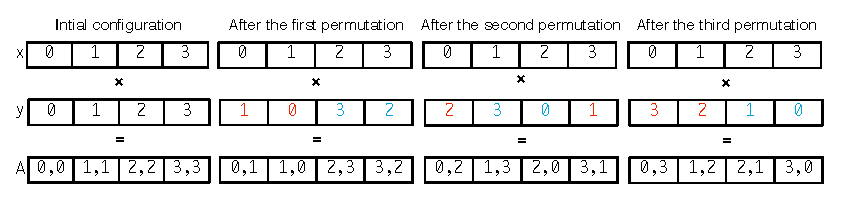
\includegraphics[scale=0.6]{coffee/pictures/vect-by-vect-inline.pdf}}
\caption{Outer-product vectorization by permuting values in a vector register.}
\label{fig:vect-by-vect}
\end{figure}

The storage layout of $A$, however, is incorrect after the application of this outer-product-based vectorization (\emph{op-vect}, in the following). It can be efficiently restored with a sequence of vector shuffles following the pattern highlighted in Figure~\ref{fig:restore-layout}, executed once outside of the \texttt{ijk} loop nest. The pseudo-code for the Burgers local assembly kernel when using \emph{op-vect} is shown in Listing~\ref{code:burgers-opvect}.

\begin{figure}
\centerline{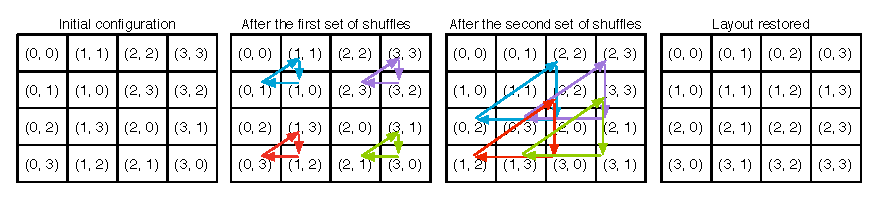
\includegraphics[scale=0.6]{coffee/pictures/vect-restore-inline.pdf}}
\caption{Restoring the storage layout after \emph{op-vect}. The figure shows how 4$\times$4 elements in the top-left block of the element matrix $A$ can be moved to their correct positions. Each rotation, represented by a group of three same-colored arrows, is implemented by a single shuffle intrinsic.}
\label{fig:restore-layout}
\end{figure}


\subsection{Exposing Matrix-Matrix Multiplications for BLAS Operations}
\label{sec:coffee-blas}

In this section, a way of systematically transforming the local element matrix computation into a sequence of matrix-matrix multiplication operations is discussed. 

If such operations could be exposed, highly-optimized dense linear algebra libraries, for instance MKL or ATLAS BLAS, could be used, which would potentially result in notable performance improvements. It is true that the basis functions' size is usually too small to obtain any gain from BLAS routines, which are tuned for large arrays~\citep{nek5000}; however, this can significantly increase with the order of the method and due to the presence of coefficient functions in the equation. Since our research is an exploration of optimization techniques for generic equations (i.e. nothing is assumed about the order of the method and the mathematical structure of the form), an algorithm capable of translating assembly expressions into a sequence of BLAS calls has been studied. The main steps of the algorithm are informally provided next. 

By fully applying the rewrite rules in Figure~\ref{fig:rewrite-rules}, an assembly expression is reduced to a summation, over each quadrature point, of outer products along the test and trial functions. Each outer product is then isolated, i.e. the assembly expression is split into chunks, each chunk representing an outer product over test and trial functions. Statements in the bodies of the surrounding loops (e.g. coefficients evaluation at a quadrature point, temporaries introduced by expression rewriting) are vector-expanded and hoisted completely outside of the loop nest, similarly to what we have described in Section~\ref{sec:expr-rewriter-obj}. This renders the loop nest perfect; that is, there is no intervening code among the various loops. The element matrix evaluation has now become a sequence of dense matrix-matrix multiplies (transposition aside)
\begin{equation*}
A_{jk} = \sum_{i} x_{0_{ij}} \cdot y_{0_{ik}} + \sum_{i} x_{1_{ij}} \cdot y_{1_{ik}} + ...
\end{equation*}
where $x0, x1, y0, y1, ...$ are tabulated basis functions or vector-expanded temporaries introduced at expression rewriting time. Eventually, the storage layout of the involved operands is changed so as to be conforming to the BLAS interface (e.g. two dimensional arrays are flatten as one dimensional arrays). The translation into a sequence of DGEMM calls is the last, straightforward step. 

\section{General-purpose Optimizations}
\label{sec:coffee-genpurp-opts}

\subsection{Loop Interchange}
All loops are interchangeable, provided that temporaries are introduced if the nest is not perfect. For the employed storage layout, the loop permutations \texttt{ijk} and \texttt{ikj} are likely to maximize performance. Conceptually, this is motivated by the fact that if the \texttt{i} loop were in an inner position, then a significantly higher number of load instructions would be required at every iteration. We tested this hypothesis in manually crafted kernels. We found that the performance loss is greater than the gain due to the possibility of accumulating increments in a register, rather than memory, along the \texttt{i} loop. The choice between \texttt{ijk} and \texttt{ikj} depends on the number of load instructions that can be hoisted out of the innermost dimension. As discussed in the next sections, a good heuristics it to choose as outermost the loop along which the number of invariant loads is smaller so that more registers remain available to carry out the computation of the local element matrix.

\subsection{Loop Unroll}
Loop unroll (or unroll-and-jam of outer loops) is fundamental to the exposure of instruction-level parallelism, and tuning unroll factors is particularly important.

We first observe that manual full (or extensive) unrolling is unlikely to be effective for two reasons. Firstly, the \texttt{ijk} loop nest would need to be small enough such that the unrolled instructions do not exceed the instruction cache, which is rarely the case: it is true that in a local assembly kernel the minimum size of the \texttt{ijk} loop nest is 3$\times$3$\times$3 (triangular mesh and polynomial order 1), but this increases rapidly with the polynomial order of the method and the discretization employed (e.g. tetrahedral meshes imply larger loop nests than triangular ones), so sizes greater than 10$\times$10$\times$10, for which extensive unrolling would already be harmful, are in practice very common. Secondly, manual unrolling is dangerous because it may compromise compiler auto-vectorization by either removing loops (most compilers search for vectorizable loops) or losing spatial locality within a vector register.

By comparison with implementations characterized by manually-unrolled loops, we noticed that recent versions of compilers like GNU's and Intel's estimate close-to-optimal unroll factors when the loops are affine and their bounds are relatively small and known at compile-time, which is the case of our kernels. Our choice, therefore, is to leave the backend compiler in charge of selecting unroll factors. The only situation in which we explicitly unroll-and-jam a loop is when the outer-product vectorization is used, since the transformed code prevents the Intel compiler from applying this optimization, even if specific pragmas are added.

%TODO: maybe we can clarify that unroll-and-jam for opvect corresponds to changing the tile size...

\section{Design and Implementation of COFFEE}
\label{sec:coffee-implementation}
\subsection{Input ad Output: the Integration with Firedrake}
\subsection{Structure}
\subsection{Conveying Domain-Specific Knowledge}

\subsection{Model-driven Dynamic Autotuning}
\label{sec:coffee-autotune}

Determining the sequence of transformations that maximizes the performance of a problem requires investigating a broad range of factors, including mathematical structure of the input form, polynomial order of employed function spaces, presence of pre-multiplying functions, and, of course, the characteristics of the underlying architecture. The set of possible optimizations is very large, so the selection problem is challenging. The sole Expression Rewriter, for instance, can generate a wide variety of implementations by just applying rewrite rules up to different extents.  

We tackle the optimizations selection problem by compiler autotuning. Not only does it allow to determine the best combination of transformations, also it enables exploring parametric low-level optimizations, such as loop unroll, unroll-and-jam, and interchange, by trying different unroll factors and loop permutations. By leveraging the cost model defined in our previous study, domain knowledge, and a set of heuristics, we manage to keep the autotuner overhead at a minimum, whilst achieving significant speed ups over the purely cost-model-based implementations in all of the forms we have evaluated. In particular, our autotuner usually requires order of seconds to determine the fastest kernel implementation, a negligible overhead when it comes to iterate over real-life unstructured meshes.

COFFEE analyzes the input problem and decides what variants it is worth testing through autotuning, as described later. Each variant is obtained by requesting specific transformations to the Expression Rewriter and the Code Specializer. The possible variants are then provided to the autotuner, in the form of abstract syntax trees. The autotuner is a template-based code generator. By inspecting an abstract syntax tree, it determines how to generate ``wrapping'' code that 1) initializes kernel's input variables with fictitious values and 2) calls the kernel. These two points are executed repeatedly in a \emph{while} loop for a pre-established amount of time (order of milliseconds). At the exit of the \emph{while} loop, the times the kernel was invoked is recorded. Eventually, the variant executed the largest number of iterations is designated as the fastest implementation. Suitable compiler directives are used to prevent inlining of all function calls: this avoids the situation in which some variants are inlined and some are not, which would fake the autotuner's output. 

The autotuning process is dynamic: depending on the complexity of the input problem, more or less variants are tried. General heuristics, which can be considered a revisited version of those presented in~\cite{nek5000}, are applied
\begin{itemize}
\item Loop permutations that are likely to worsen the performance are excluded from the search space. According to the cost model, and for the same reasons explained in~\cite{Luporini}, we enable only variants in which the loop over quadrature points is either the outermost or the innermost. This is due to the fact that versions of the code in which such loop lies between the test and trial functions loops are typically lower performing.
\item The unroll factors must divide the loop bounds evenly to avoid the introduction of reminder (scalar) loops.
\item The innermost loop is never explicitly unrolled. This is because we expect auto-vectorization along this loop, so memory accesses should be kept unit-stride. 
\end{itemize}
The autotuner is also domain-aware: the following heuristics, which capture properties of the computational domain, are exploited
\begin{itemize}
\item The lengths of test and trial functions loops are identical in some cases, for example when they originate from the same function space. In such cases, since for the employed storage layout the memory access pattern is symmetrical along these two loops, we prune their interchange from the search space. 
\item The larger is the polynomial order of the method, the larger is the assembly loop nest. In these cases, we impose a bound on the loop nest's overall unroll factor (which we found empirically) to avoid uselessly testing too many unroll factors. 
\item On the other hand, if the polynomial order is low, i.e. when the loop nest is small, we prune variants that we know will be low-performing, e.g. those resorting to BLAS.
\item We specifically select two levels of expression rewriting. In the ``base'' level, only generalized loop-invariant code motion, as described in~\cite{Luporini}, is applied. This means that only a subset of the rewrite rules exposed in~\ref{fig:rewrite-rules} will be considered. In the ``aggressive'' level, all of the rewrite rules are applied. Many other trade-offs, which we do not explore, would be feasibile, however. 
\item For the expression splitting optimization described in~\cite{Luporini} and summarized in Section~\ref{sec:summary-opts}, we test only three split factors, namely 1, 2, 4. Also, if the input problem uses mixed function spaces, the iteration space is already split at expression rewriting time to avoid computation over zero-valued columns; in these cases, we do not further apply expression splitting.
\item Based on the cost model, the padding and data alignment optimization is always applied. 
\end{itemize}

All of the previous points contribute to minimize the overhead of the autotuning process. We will discuss the actual cost of autotuning in Section~\ref{sec:coffee-pereval-autotune}.

\section{Performance Analysis}
\subsection{Contribution of Individual Optimizations}
\label{sec:coffee-perfeval-single}
\subsection{Evaluation in Forms of Increasing Complexity}
\subsection{Details on the Autotuning Process}
\label{sec:coffee-pereval-autotune}

\subsection{Full Application Study}


\section{Related Work}
\label{sec:coffee-related-work}

\section{Generality of the Approach and Applicability to Other Domains}
\label{sec:generality}

\section{Conclusion}